\chapter{System Implementation}
\label{chap:implementation}

This chapter presents the practical implementation of the proposed phishing
URL detection system. It explains how the data-processing pipeline,
classifiers, GAN augmentation, hybrid model, and browser extension were joined
into one working system. Detailed source-code descriptions are omitted because
the purpose of this chapter is to describe the implemented system rather than
individual programming instructions.

\section{Implementation Overview}

The project was implemented mainly in Python. PyTorch was used for the neural
networks and GANs, while scikit-learn was used for the Random Forest (RF) and
Support Vector Machine (SVM) baselines. Neural training was performed using an
NVIDIA RTX~3060 Laptop GPU through CUDA. The browser extension was implemented
in JavaScript using the Chromium Manifest~V3 standard, and the selected model
was converted to ONNX for local browser inference.

The implementation followed the experimental method established in
Chapter~\ref{chap:methodology}. Data preparation, model training, GAN
generation, evaluation, and browser deployment were kept as separate stages.
This separation made it possible to repeat an experiment without changing the
frozen training and evaluation data.

\begin{table}[htbp]
\centering
\caption{Main technologies used in the implemented system.}
\label{tab:implementation-software}
\small
\begin{tabular}{@{}p{0.28\textwidth}p{0.27\textwidth}p{0.35\textwidth}@{}}
\toprule
Part & Technology & Main purpose \\
\midrule
Data processing & Python, SQLite, NumPy & Cleaning, splitting, encoding, and storing URLs \\
Traditional classifiers & scikit-learn & RF and SVM training and evaluation \\
Neural models and GANs & PyTorch and CUDA & CNN, RNN, LSTM, hybrid, and GAN training \\
Result production & JSON, CSV, Matplotlib & Saving metrics and producing graphs \\
Browser deployment & JavaScript and ONNX Runtime Web & Local URL classification in the browser \\
Extension platform & Chromium Manifest V3 & Navigation monitoring, warnings, and local feedback \\
\bottomrule
\end{tabular}
\end{table}

\section{Project Structure}

The earlier experiments were preserved as Version~1 and Version~2. Version~3
contains the final organised implementation. Its main folders separate source
code, prepared data, trained models, experimental results, graphs, and the
browser extension. This organisation prevents an old checkpoint or dataset
from being confused with the final experimental materials.

The main experimental settings are stored in a central configuration. These
settings include the data split, URL length, model dimensions, batch sizes,
training limits, random seeds, and GAN augmentation ratios. Therefore, the
important settings remain consistent across repeated runs. Each completed run
also records the model, seed, dataset identity, selected threshold, and final
metrics.

\section{Data Preparation}

The selected multi-source dataset was processed into one controlled dataset for
classifier training and evaluation. Each input URL was assigned a binary label:
legitimate or phishing. Invalid labels, malformed entries, duplicate URLs, and
conflicting records were removed or placed in a quarantine record instead of
being silently accepted.

URLs were normalised before splitting. This included removing unnecessary
spaces, standardising the hostname, handling the scheme consistently, and
checking the port and URL structure. The normalised hostname was then used to
create deterministic training, validation, and test partitions. Keeping the
same hostname in one partition reduces identity leakage and provides a more
meaningful internal evaluation.

The character vocabulary was built from the permitted training data. Every URL
was converted into a fixed-length sequence of 128 character identifiers. The
prepared arrays were stored in a form that could be read efficiently during
training. Human-readable manifests and dataset hashes were also saved so that
the origin and identity of the rows could be checked later.

\section{Feature Extraction}

Two representations of a URL were used in the project. The first was the raw
character sequence, which allowed neural networks to learn local combinations
of letters, digits, and symbols. The second was a set of 35 lexical and
structural measurements used by the final hybrid model.

The lexical features describe properties such as URL length, hostname length,
path and query length, number of dots and subdomains, digits, hyphens, special
characters, entropy, suspicious terms, IP-address use, and domain-suffix
structure. Exact domain identities were not used as input features. Numerical
features were scaled using values learned only from the training partition, and
the same stored values were later used during testing and browser inference.

This combination was selected because the character representation can learn
patterns directly from URL text, while the lexical representation provides
explicit structural information. The complete feature definitions and their
research purpose were presented in Chapter~\ref{chap:methodology}.

\section{Classifier Implementation}

The implemented baselines were RF, SVM, CNN, RNN, and LSTM. RF and SVM used
the lexical representation, whereas the neural baselines used the encoded
character sequence. These models provided different comparison families rather
than several minor variations of the same algorithm.

The final hybrid classifier contains two branches. The first is a
character-level CNN that learns patterns directly from the URL string. The
second is a small neural branch that processes the 35 lexical features. Their
learned representations are combined before the final phishing probability is
produced. This design permits the classifier to use both automatically learned
text patterns and explicit URL structure.

\begin{table}[htbp]
\centering
\caption{Implemented classifiers and their input representations.}
\label{tab:implemented-classifiers}
\small
\begin{tabular}{@{}p{0.19\textwidth}p{0.28\textwidth}p{0.43\textwidth}@{}}
\toprule
Classifier & Input & Role in the study \\
\midrule
RF & Lexical features & Non-linear traditional baseline \\
SVM & Lexical features & Linear margin-based baseline \\
CNN & URL characters & Learns short local character patterns \\
RNN & URL characters & Recurrent sequence baseline \\
LSTM & URL characters & Recurrent model with longer memory \\
Hybrid & Characters and lexical features & Final combined classifier and deployment candidate \\
\bottomrule
\end{tabular}
\end{table}

All models followed the same experimental partitions and registered random
seeds. Neural models used class-aware loss weighting, validation-based early
stopping, and GPU training. The best validation checkpoint was retained rather
than automatically using the last epoch. Decision thresholds were selected
from validation data and then frozen before testing. The test data were used
only for the final measurement of a completed condition.

\section{GAN Implementation and Augmentation}

The project implemented multiple URL-generating GAN approaches during its
development, including SeqGAN, RelGAN, URL-GAN, and the final multi-source
hard-example GAN configuration (MS-HardGAN-C). These generators were trained
using phishing URLs from the training partition only. Their purpose was to
learn phishing-like character patterns and produce additional candidate URLs;
they were not treated as systems capable of predicting future attacks.

Training began with a supervised sequence-learning stage so that a generator
could first learn valid URL structure. Adversarial training was then introduced:
the discriminator learned to distinguish real phishing URLs from generated
ones, while the generator learned to produce more realistic outputs. The final
hard-example configuration additionally used frozen classifiers to identify
generated samples that were difficult for more than one classifier family.

Generated URLs were not added directly to the training set. They first passed
validity, realism, uniqueness, and overlap checks. Obvious formatting errors,
duplicates, copies of real training URLs, and unsuitable structural outliers
were rejected. The accepted URLs formed frozen synthetic pools from which the
registered augmentation percentages were created.

The real-only and augmented conditions retained the same real training rows.
Their only intended difference was the addition of the selected synthetic
phishing URLs. This controlled design allowed later comparisons to measure the
effect of GAN augmentation rather than a change in the underlying real data.

For the direct SeqGAN--MS-HardGAN-C comparison, SeqGAN was retrained from
scratch on the exact 84,280 phishing token rows used by MS-HardGAN-C. SeqGAN
completed five supervised language-model epochs and three adversarial epochs,
then produced 500,000 candidates. The standard filters accepted 344,507 URLs;
the accepted pool had 100\% uniqueness and validity and no exact accepted
memorisation. After a second overlap check against the complete HYB-MS real
training pool, exactly 40,410 URLs were frozen for the 10\% condition. New
HYB-MS models were trained for seeds 42, 43, and 44. The MS-HardGAN-C models
used the matching real-row count, synthetic-row count, architecture, sampler,
features, and threshold-selection rule. Separate output directories preserved
the earlier models and results.

\section{Training and Evaluation Process}

Figure~\ref{fig:implementation-flow} summarises the complete implemented flow.
The real data are prepared once and used for classifier training. The phishing
training subset also supplies the GANs. Accepted generated URLs are combined
with the same real training partition to form the augmentation conditions.
Real-only and augmented models are then evaluated using unchanged internal and
external datasets.

\begin{figure}[htbp]
\centering
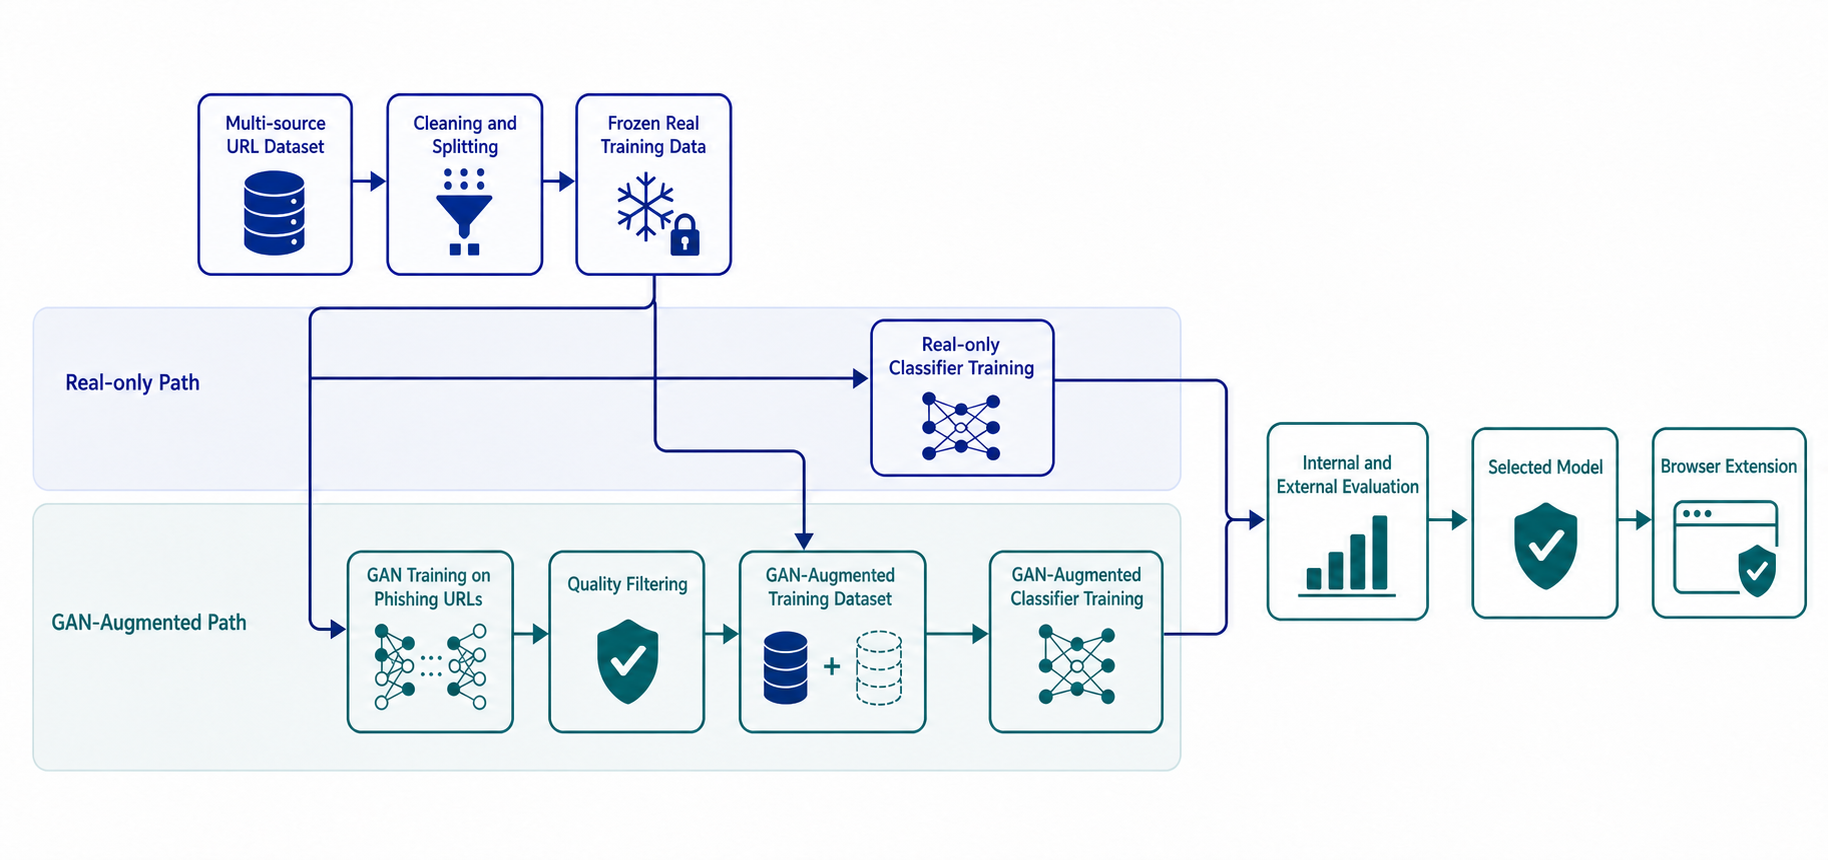
\includegraphics[width=\textwidth]{figure_5_1_system_workflow.png}
\caption{Parallel real-only and GAN-augmented training, evaluation, and deployment workflow.}
\label{fig:implementation-flow}
\end{figure}

For every evaluation, the system stored the confusion matrix and the required
metrics: accuracy, precision, recall, F1-score, ROC-AUC, false-positive rate
(FPR), and false-negative rate (FNR). PR-AUC was also stored where relevant.
Results across seeds were summarised using the mean and standard deviation.
External evaluation reused the frozen model and threshold without retraining.

Model checkpoints, experiment settings, predictions, metrics, and training
histories were saved for traceability. Tables and graphs were produced from
these stored files rather than copied manually from terminal output. The full
experimental results are presented in the next chapter.

\section{Browser Extension Implementation}

The selected three-seed hybrid ensemble was converted from PyTorch to ONNX and
included in the browser extension. The extension performs inference locally,
so ordinary URL classification does not require a remote prediction server.
The Python and JavaScript preprocessing outputs were compared before the model
bundle was accepted, ensuring that the browser receives the same character and
lexical representations used during evaluation.

When a user navigates to a page, the extension normalises the URL, calculates
its features, obtains the ensemble score, and applies the selected warning
policy. The interface supports non-blocking caution messages, a secondary
review state, and an interrupting warning for the highest-risk decisions. A
passive demonstration mode reports the decision without redirecting the user.
Trusted sites and IP-address inputs are handled separately to reduce avoidable
false alarms.

Repeated browser events can otherwise cause one page to be scanned many times.
The extension therefore prevents simultaneous duplicate scans and reuses a
recent result for the same tab and URL. For user evaluation, a canonical URL is
counted once as a unique observation, while repeated events are recorded only
as technical reliability information.

\section{Local Feedback and Privacy}

A separate user-evaluation build was created without replacing the stable
extension. Participants must agree before local study counters begin. The
extension does not automatically upload browsing history. Instead, results are
stored on the participant's device and can be exported voluntarily after the
evaluation.

Users can report a false positive when a legitimate page receives an incorrect
phishing warning, or a false negative when a phishing page is not warned about
appropriately. A URL is stored only when the participant explicitly submits a
feedback report. Query values and fragments are removed before export to reduce
the chance of including personal information. The exported summary contains
decision counts, warnings, errors, timing information, and the submitted
feedback required for the evaluation.

\section{Verification and Reproducibility}

Automated checks were used for dataset integrity, preprocessing, feature
dimensions, model inputs, metric calculations, browser policy, duplicate-scan
handling, and agreement between PyTorch and ONNX predictions. Important data
and model files were identified by hashes, and experiment outputs were stored
under separate condition and seed directories.

These controls do not guarantee that every future URL distribution will match
the research data. They do, however, ensure that the reported experiments can
be traced to specific datasets, settings, checkpoints, and thresholds. This is
necessary for a fair comparison between real-only and GAN-augmented models.

\section{Chapter Summary}

The proposed system was implemented as an organised pipeline connecting data
preparation, baseline classifiers, a hybrid classifier, GAN-based URL
augmentation, controlled evaluation, and browser deployment. The final hybrid
model combines character-level CNN learning with lexical URL features, while
the GAN stage supplies filtered synthetic phishing examples for controlled
augmentation experiments.

The selected ensemble was exported to ONNX and integrated into a Manifest~V3
extension that performs local inference, presents tiered warnings, reduces
duplicate scans, and supports consent-based local feedback. The following
chapter reports the internal, augmentation, external, and threshold results
produced by this implementation. Browser operation and user evaluation are
then presented separately in Chapter~7.
